%%=============================================================================
%% Proof of concept
%%=============================================================================

\chapter{Proof of concept}
\label{ch:POC}

Als proof of concept worden er 2 zaken van Skedify uitgewerkt in een EventSourced systeem. Het eerste is het maken van een afspraak (appointment) en het tweede het wijzigen van een appointment (reschedulen).

De proof of concept is gemaakt in de programmeertaal PHP, dit omdat Skedify ook geschreven is in PHP. Via deze weg zitten we dichter bij de realiteit, en moeten er ook geen andere programmeertalen vergeleken worden met elkaar.

Het blijkt dat de setup van deze proof of concept zeer veel met zich mee bracht, zoals het maken van de EventStore, het bepalen van de aggregates en de Domain Events. Het is wel zo dat de \Glspl{command} en \Glspl{query} een duidelijke 1-op-1 mapping zijn met de businesskant. Dit werd als positief aanschouwd door de product owner van Skedify, Christophe Thelen.

De testbaarheid van \Glspl{command} en Domain Events gingen zeer vlot met als bonus dat er documentatie van van deze testen gegenereerd konden worden (zoals te zien in figuur~\ref{fig:documentation}).

\begin{figure}[h]
\caption{Gegenereerde documentatie van de geautomatiseerde testen} \label{fig:documentation}
\centering
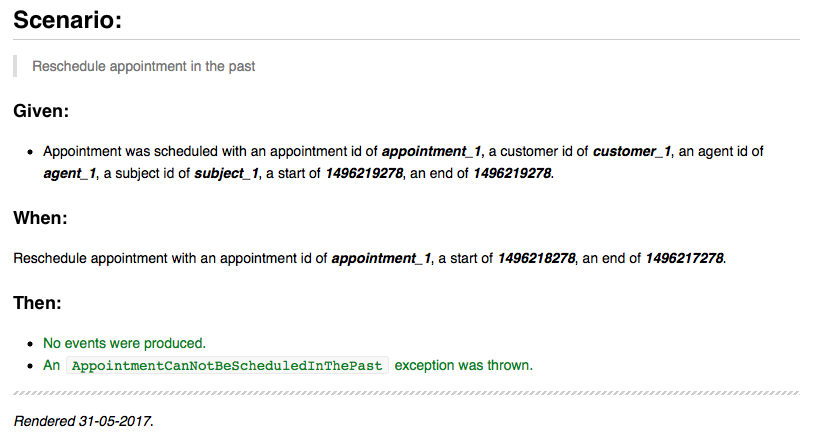
\includegraphics[width=0.9\textwidth]{img/documentatie-voorbeeld}
\end{figure}

De proof of concept kan teruggevonden worden via \textcite{malfait2017poc}.